%%%%%%%%%%%%%%%%%%%%%%%%%%%%%%%%%%%%%%%%%%%%%%%%%%%%%%%%%%%%%%%%%%%%%%%%%%%%%%%%%%%%%%
% ---------------------------------------------------------------------------------  %
% ---------------------------------------------------------------------------------  %
%                                                                                    %
%                  MODELO DE MONOGRAFIA DO E-COMP - POLI - UPE                       %
%                                                                                    %
% ---------------------------------------------------------------------------------  %
% ---------------------------------------------------------------------------------  %
%%%%%%%%%%%%%%%%%%%%%%%%%%%%%%%%%%%%%%%%%%%%%%%%%%%%%%%%%%%%%%%%%%%%%%%%%%%%%%%%%%%%%%

\chapter{Resultados} \label{cap:resultados} 
Na Tabela \ref{tab:tabela_taxa_acertos} s�o mostrados a m�dia e desvio padr�o (entre par�nteses) dos resultados dos seis experimentos descritos na Se��o \ref{sec:configuracao_classificador}. As configura��es da rede podem ser observadas na Tabela \ref{tab:tabela_configuracoes}. Todos os resultados s�o expostos mais claramente na Figura \ref{fig:taxa_classificacao}, onde est�o repreentados os \emph{boxplots} das taxas de classifica��o em fun��o da configura��o da MLP.

\begin{table}[htbp]
\centering
\textbf{
	\caption{Resultados MLP}
	\label{tab:tabela_taxa_acertos}
}
\begin{tabular}{ c c c }
	\hline
	\textbf{Configura��o} & \textbf{Grafo com \emph{Stopwords}} & \textbf{Grafo sem \emph{Stopwords}}\\
	\hline
	1 & 52,70(10,03) & 47,96(9,86) \\
	2 & 51,56(9,13)  & 47,61(7,85) \\
	3 & 49,03(7,67)  & 46,55(9,10) \\
	4 & 40,77(12,08) & 34,87(11,56) \\
	5 & 38,36(13,61) & 34,05(14,79) \\
	6 & 36,87(13,68) & 29,57(12,16) \\
	\hline
\end{tabular}
\end{table}

\begin{table}[htbp]
	\centering
	
	\textbf{
		\caption{Configura��es da MLP}
		\label{tab:tabela_configuracoes}
	}	
	\begin{tabular}{ c c c }
		\hline
		\textbf{Configura��o} & \textbf{N�mero de Camadas} & \textbf{N�mero de Neur�nios}\\
		\hline
		1 & 1 & $\left[ 10 \right]$ \\
		2 & 1 & $\left[ 20 \right]$ \\
		3 & 1 & $\left[ 5 \right]$ \\
		4 & 2 & $\left[ 10, 10 \right]$ \\
		5 & 2 & $\left[ 20, 20 \right]$ \\
		6 & 2 & $\left[ 5, 5 \right]$ \\
		\hline
	\end{tabular}
\end{table}

\begin{figure}[htpb]
	\begin{center}
		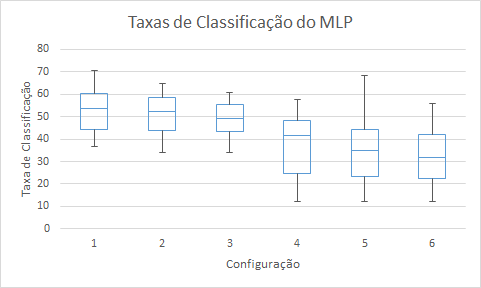
\includegraphics[width=400pt]{imagens/classificacao_mlp.png}
		\textbf{
			\caption{
				\emph{Boxplots} das configura��es da MLP
			}
			\label{fig:taxa_classificacao}
		}
	\end{center}
\end{figure}

\begin{table}[htbp]
	\centering
	
	\textbf{
		\caption{Matriz de confus�o para uma execu��o da MLP em configura��o 1 com escore 52,94\%}
		\label{tab:matriz_de_confusao}
	}	
	\begin{tabular}{ c c c c c c c c c }

		& HHM & ACD & EAP & BS & CD & TH & MT & PGW  \\
		HHM & 36 & 4 & 3 & 5 & 2 & 0 & 1 & 0 \\
		ACD & 16 & 9 & 5 & 7 & 3 & 2 & 1 & 8  \\
		EAP & 4 & 3 & 38 & 2 & 2 & 0 & 1 & 1  \\
		BS & 4 & 6 & 0 & 35 & 3 & 2 & 0 & 1  \\
		CD & 2 & 0 & 7 & 2 & 21 & 3 & 16 & 0  \\
		TH & 2 & 4 & 4 & 2 & 7 & 16 & 51 & 11  \\
		MT & 1 & 2 & 1 & 1 & 15 & 3 & 24 & 4  \\
		PGW & 0 & 2 & 0 & 2 & 0 & 6 & 4 & 37  \\
		
	\end{tabular}
\end{table}

\par
Os resultados sugerem que a remo��o das \emph{stopwords} compromete a capacidade da rede de representar caracter�sticas estil�sticas. A matriz de confus�o mostrada na Tabela \ref{tab:matriz_de_confusao} pode indicar que naturalmente existem autores cujos tra�os de estilo n�o s�o bem capturados pela rede. � o caso de Arthur Conan Doyle e Thomas Hardy, que foram muito confundidos com Hector Hugh Munro e Mark Twain respectivamente.
